
\documentclass[x11names,svgnames]{beamer}

\usetheme{metropolis}
\setbeamercolor{block title}{fg=LightSkyBlue4}
\usepackage{fontspec}
\usepackage[francais]{babel}
\usepackage[french, frenchkw]{algorithm2e}
\SetKwFor{Pc}{Pour chaque}{faire}{fin}
\SetKwProg{Fn}{Fonction}{:}{}
\usepackage{textcomp}
\usepackage{minted}
\usepackage{xspace}
\usepackage{amsmath}
\usepackage{mathtools}
\usepackage{marvosym}
\usepackage[framemethod=TikZ]{mdframed}
\usepackage{tikz}
\usetikzlibrary{calc, positioning, arrows, decorations.pathmorphing}
% https://tex.stackexchange.com/questions/401884/how-do-i-change-hyperlinks-color-only
\hypersetup{
  colorlinks,
  allcolors=.,
  urlcolor=DarkBlue,
  pdftitle={AP1 - 13 novembre 2023 - CC1 et récursivité}
}


\author{}
\date{Lundi 13 novembre 2023}

\title{
\includegraphics[width=0.75\textwidth]{../../../img/logo-igm.png} \\ Algorithmique et Programmation 1}
\institute{L1 Mathématiques - L1 Informatique \\ Semestre 1}

\begin{document}

\maketitle

\begin{frame}{CC1}

Moyenne : 12,7/20 \qquad Médiane : 14/20

\begin{figure}[ht]
  \centering
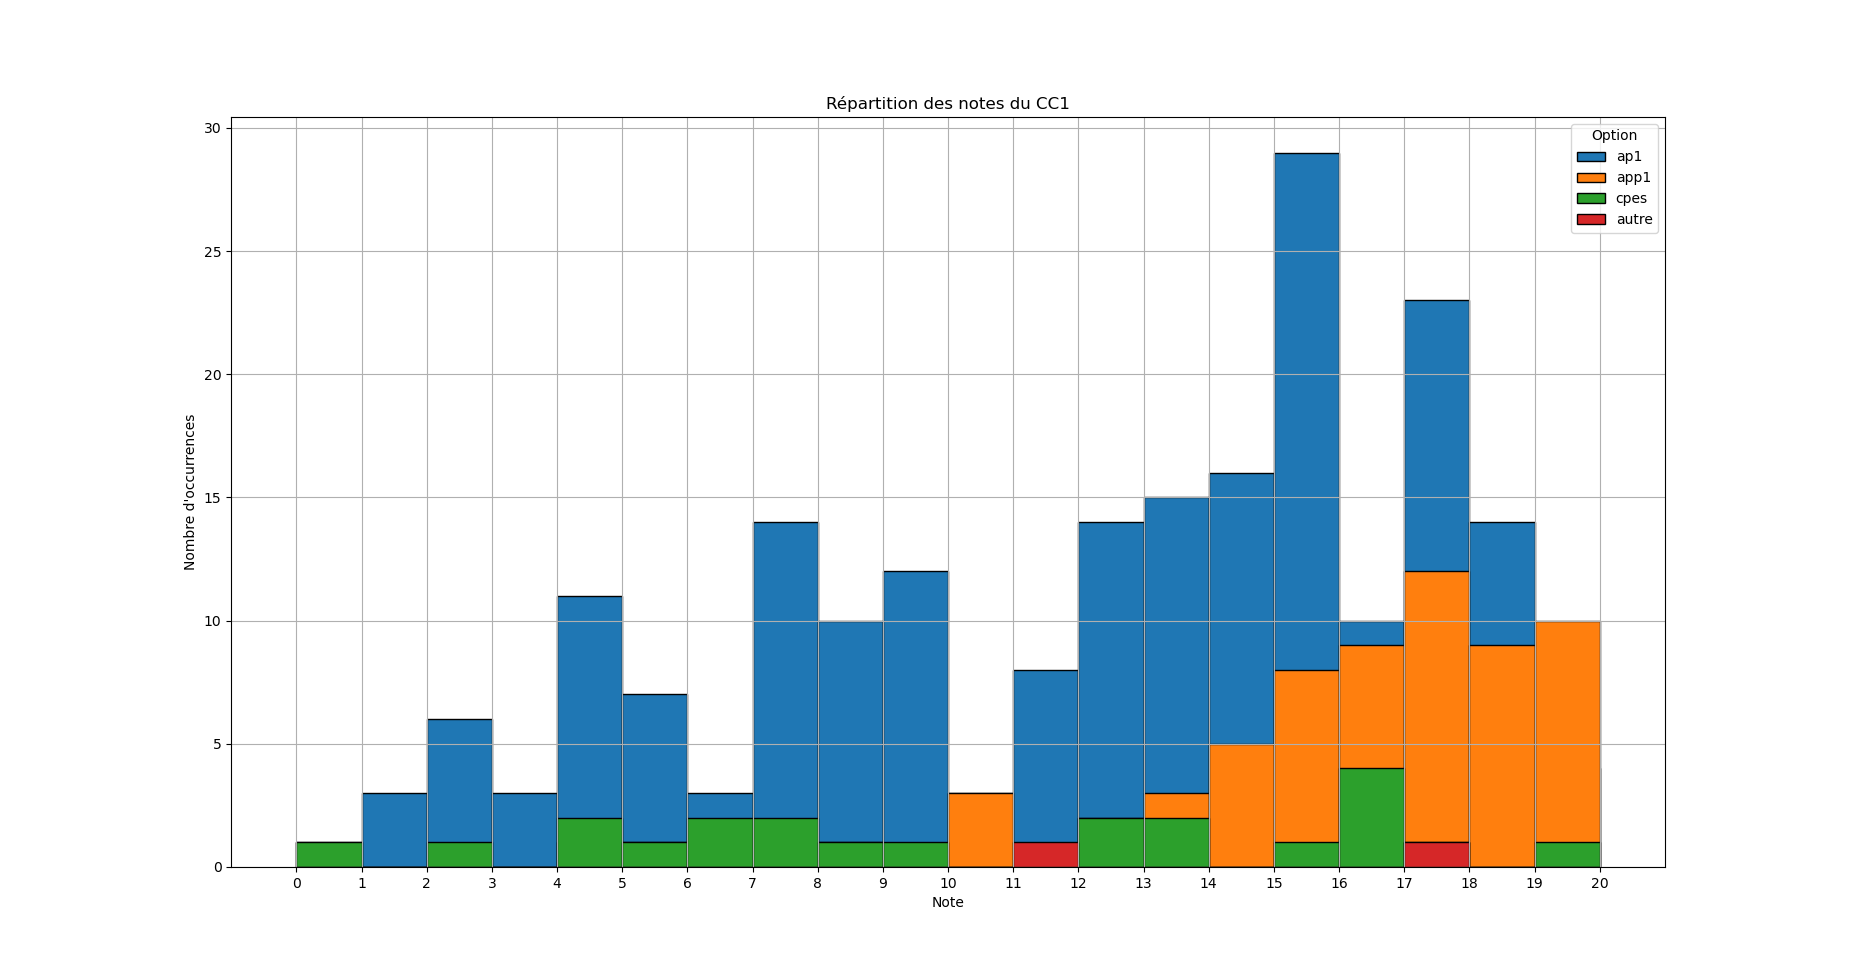
\includegraphics[width = \textwidth]{img/Stats_CC1.png}
\end{figure}

\end{frame}




\section{Dictionnaires}

\begin{frame}[fragile]
  \frametitle{Exemple : Regrouper les informations d'un joueur}

  On veut modéliser un jeu à plusieurs joueurs, où les joueurs ont :
  \begin{itemize}
  \item Un pseudo
  \item Une couleur
  \item Un score
  \end{itemize}


  On peut bien sûr utiliser des listes :
  \begin{mdframed}[roundcorner=5pt]
\begin{minted}{python}
pseudos = ["aze89", "yoplait", "azareth"]
couleurs = ["red", "yellow", "green"]
scores = [0, 0, 0]
\end{minted}
  \end{mdframed}
  \pause
  Mais :
  \begin{itemize}
\item Il faut se trimballer trois listes
\item Et ne pas se planter quand on ajoute un joueur
\item Ou une caractéristique
  \end{itemize}
\end{frame}

\begin{frame}[fragile]
  \frametitle{Exemple : Regrouper les informations d'un joueur}

  Groupons donc par joueur :
  \begin{mdframed}[roundcorner=5pt]
\begin{minted}{python}
joueur1 = ["qsdf89", "red", 25]
joueur2 = ["yoplait", "yellow", 20]
joueur3 = ["azerath", "green", 28]
joueurs = [joueur1, joueur2, joueur3]
\end{minted}
  \end{mdframed}
  \pause
  Mais il faut se rappeler que :
  \begin{itemize}
\item 0 correspond au pseudo
\item 1 correspond à la couleur
\item 2 correspond au score
  \end{itemize}

  On aimerait donc donner un nom à chaque indice !
\end{frame}


\begin{frame}[fragile]
  \frametitle{Exemple : Regrouper les informations d'un joueur}

C'est précisément ce que font les dictionnaires !

  \begin{mdframed}[roundcorner=5pt]
\begin{minted}{python}
joueur1 = {'pseudo': 'qsdf89',
           'couleur': 'red',
           'score': 25}
joueur2 = {'pseudo': 'yoplait',
           'couleur': 'yellow',
           'score': 20}
joueur3 = {'pseudo': 'azerath',
           'couleur': 'green',
           'score': 28}
joueurs = [joueur1, joueur2, joueur3]
\end{minted}
  \end{mdframed}
  Les dictionnaires permettent ainsi de rassembler plusieurs informations concernant une personne.
\end{frame}

\begin{frame}[fragile]
  \frametitle{Les dictionnaires}

\textbf{Dictionnaire :} objet associant une liste de clés à des valeurs.

\begin{itemize}
      \item Entrées/clés (\emph{keys}) : d'un type de base \emph{immutable}
      \item Valeurs associées (\emph{values}) : de n'importe quel type
      \item Les paires (clé, valeur) sont appelées \emph{objets} (\emph{items})
      \end{itemize}

Un objet de type \mintinline{python}{dict} est :
\begin{itemize}
\item \textbf{une collection}
\item \textbf{mutable}
\item \textbf{hétérogène} (peut contenir des types différents)
\item \textbf{itérable} (utilisable dans un \mintinline{python}{for})
\end{itemize}

\end{frame}

\begin{frame}[fragile]
  \frametitle{Fonctions de base}

  \begin{block}{Créer un dictionnaire}
  \begin{mdframed}[roundcorner=5pt]
\begin{minted}{python}
# Pour créer un dictionnaire vide
dictionnaire = dict()  # Ou bien
dictionnaire = {}
# Pour l'initialiser avec des valeurs :
# voir précédemment
\end{minted}
  \end{mdframed}
  \end{block}

  \begin{block}{Accéder à une valeur via sa clé}
  \begin{mdframed}[roundcorner=5pt]
\begin{minted}{python}
dictionnaire[cle]
\end{minted}
  \end{mdframed}
  \end{block}

  \begin{block}{Modifier une valeur}
  \begin{mdframed}[roundcorner=5pt]
\begin{minted}{python}
dictionnaire[cle] = valeur
\end{minted}
  \end{mdframed}
\end{block}
\end{frame}

\begin{frame}[fragile]{Fonctions de base}
  \begin{exampleblock}{Exemple}
  \begin{mdframed}[roundcorner=5pt]
\begin{minted}{python}
joueur1 = {'pseudo': 'qsdf89',
           'couleur': 'red',
           'score': 25}
print(joueur1['couleur'])  # red
joueur1['score'] += 3
print(joueur1['score'])  # 28
\end{minted}
    \end{mdframed}
\pause
  \begin{mdframed}[roundcorner=5pt]
\begin{minted}{python}
joueur1['ville'] = 'Champs'
print(joueur1)
# {'pseudo': 'qsdf89', 'couleur': 'red',
#  'score': 28, 'ville': 'Champs'}
\end{minted}
    \end{mdframed}
\end{exampleblock}
\end{frame}

\begin{frame}[fragile]
  \frametitle{Les éléments du dictionnaire : les clés (\emph{keys})}

    On peut accéder à l'ensemble des clés du dictionnaire :
  \begin{mdframed}[roundcorner=5pt]
\begin{minted}{python}
dictionnaire.keys()
\end{minted}
  \end{mdframed}
    On peut donc tester si une clé est dans le dictionnaire :
  \begin{mdframed}[roundcorner=5pt]
\begin{minted}{python}
if cle in dictionnaire.keys():
\end{minted}
  \end{mdframed}
  C'est la même chose d'écrire (et on préfère) :
  \begin{mdframed}[roundcorner=5pt]
\begin{minted}{python}
if cle in dictionnaire:
\end{minted}
  \end{mdframed}
  On peut aussi \alert{itérer} sur le dictionnaire :
  \begin{mdframed}[roundcorner=5pt]
\begin{minted}{python}
for cle in dictionnaire:
# C'est pareil que (mais on préfère la version courte) :
for cle in dictionnaire.keys():
\end{minted}
  \end{mdframed}
  \end{frame}

\begin{frame}[fragile]
  \frametitle{Les éléments du dictionnaire : les valeurs (\emph{values})}

    On peut accéder à l'ensemble des valeurs du dictionnaire :
  \begin{mdframed}[roundcorner=5pt]
\begin{minted}{python}
dictionnaire.values()
\end{minted}
  \end{mdframed}
    On peut donc tester si une valeur est dans le dictionnaire :
  \begin{mdframed}[roundcorner=5pt]
\begin{minted}{python}
if cle in dictionnaire.values():
\end{minted}
  \end{mdframed}
  On peut aussi \alert{itérer} sur \emph{les valeurs} du dictionnaire :
  \begin{mdframed}[roundcorner=5pt]
\begin{minted}{python}
for cle in dictionnaire.values():
\end{minted}
  \end{mdframed}
  \end{frame}

\begin{frame}[fragile]
  \frametitle{Les éléments du dictionnaire : les objets (\emph{items})}

    Enfin, on peut accéder à l'ensemble des objets du dictionnaire :
  \begin{mdframed}[roundcorner=5pt]
\begin{minted}{python}
dictionnaire.items()
\end{minted}
  \end{mdframed}
    On peut donc tester si une couple (clé, valeur) est dans le dictionnaire :
  \begin{mdframed}[roundcorner=5pt]
\begin{minted}{python}
if (cle, valeur) in dictionnaire.items():
# C'est pareil que d'écrire (et on préfère)
if dictionnaire[cle] == valeur
\end{minted}
  \end{mdframed}
  On peut aussi \alert{itérer} sur \emph{les objets} du dictionnaire :
  \begin{mdframed}[roundcorner=5pt]
\begin{minted}{python}
for (cle, valeur) in dictionnaire.items():
\end{minted}
  \end{mdframed}

  Voir aussi le \href{https://mybinder.org/v2/gh/UGE-IGM/amphis-AP1/main?labpath=2023-2024%2F7-dictionnaires%2F7-dictionnaires.ipynb}{Jupyter Notebook}.
\end{frame}

\begin{frame}
  \frametitle{Une autre application : un problème de comptage}
  
  Liste de prénoms américains (avec doublons) : quel est le plus courant ?

  \MVRightarrow{} Écrire un programme qui renvoie une liste de tuples \mintinline{python}{(prenom, nombre_occurrences)}.

  \vspace{-1em}

  \pause

  \begin{overprint}
    \onslide<2>
    \begin{block}{Première approche}
      \vspace{0.5em}
    \begin{itemize}
    \item Déterminer la liste des prénoms sans doublons
    \item Pour chaque prénom dans cette liste, compter combien de fois il apparaît
    \end{itemize}
  \end{block}
\onslide<3->
  \begin{block}{Deuxième approche}
    \vspace{0.5em}
    \begin{itemize}
    \item Créer une liste vide \mintinline{python}{occurrences}
    \item Parcourir la liste des prénoms (avec doublons)
    \item Pour chaque prénom \mintinline{python}{prenom} :
      \begin{itemize}
      \item S'il n'apparaît pas dans \mintinline{python}{occurrences}, y ajouter une liste \mintinline{python}{[prenom, 1]}
      \item S'il apparaît déjà dans \mintinline{python}{occurrences}, ajouter 1 au nombre d'occurrences correspondant
      \end{itemize}
    \end{itemize}
  \end{block}
\end{overprint}
\onslide<4>{C'est pénible\dots{} Est-ce qu'on peut faire mieux ?}
\end{frame}

\begin{frame}
  \frametitle{Le problème de comptage avec des dictionnaires}
  Liste de prénoms américains (avec doublons) : quel est le plus courant ?

  \begin{overprint}
    \onslide<1>
  \MVRightarrow{} Écrire un programme qui renvoie un dictionnaire contenant les occurrences de chaque prénom.

  \begin{itemize}
  \item Créer un dictionnaire vide \mintinline{python}{occurrences}
  \item Parcourir la liste des prénoms (avec doublons)
  \item Pour chaque prénom \mintinline{python}{prenom} :
    \begin{itemize}
    \item S'il n'apparaît pas dans \mintinline{python}{occurrences}, y ajouter une entrée \mintinline{python}{prenom : 1}
    \item S'il apparaît déjà dans \mintinline{python}{occurrences}, ajouter 1 au nombre d'occurrences correspondant
    \end{itemize}
  \end{itemize}
  \onslide<2>
  \MVRightarrow{} Écrire un programme qui détermine quels sont les prénoms utilisés.

  \begin{itemize}
  \item Calculer le dictionnaire des occurrences
  \item Afficher ses clés une par une.
  \end{itemize}
  \onslide<3>
  \MVRightarrow{} Écrire un programme qui détermine quel est le prénom le plus courant.
  \begin{itemize}
  \item Calculer le dictionnaire des occurrences
  \item Parcourir ses paires (clé, valeur) pour déterminer la clé ayant la plus grande valeur
  \end{itemize}
\end{overprint}
\end{frame}


\begin{frame}{Comment ça marche ?}
\begin{block}{Les tables de hachage}
  \vspace{0pt}
  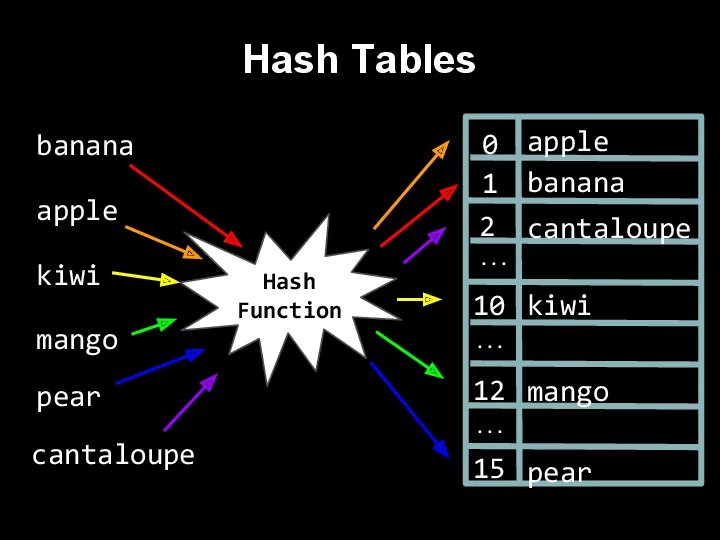
\includegraphics[height=0.6\textheight]{img/hashtable.png}
\end{block}

\begin{block}{Restrictions sur les clés}
  \vspace{0pt}
  Les clés doivent être \emph{hashables}. En pratique : d'un type de base \emph{immutable}.
\end{block}
\end{frame}



\section{Les fichiers}

\begin{frame}{Itérables (encore une fois)}

  \begin{block}{Définition}
    \vspace{0pt}
    Un objet dont on peut parcourir les éléments.
    \begin{itemize}
    \item[\MVRightarrow{}] Les dictionnaires \mintinline{python}{dict}
    \item[\MVRightarrow{}] Les intervalles \mintinline{python}{range}
    \item[\MVRightarrow{}] Les listes \mintinline{python}{list}
    \item[\MVRightarrow{}] Les chaînes de caractères \mintinline{python}{str}
    \item[\MVRightarrow{}] Les tuples \mintinline{python}{tuple}
    \item Les ensembles \mintinline{python}{set}
    \item \alert{Les fichiers \mintinline{python}{file}}
    \end{itemize}
  \end{block}
\end{frame}

\begin{frame}[fragile]{Un système de sauvegarde}

  Quand on quitte un jeu, les données en mémoire de Python sont perdues. Comment faire ?

  \pause

  Écrire dans un fichier !

  \begin{mdframed}[roundcorner=5pt]
\begin{minted}{python}
def sauvegarde(pseudos, fichier):
    f = open('pseudos.txt', 'w')  # w = write
    for pseudo in pseudos:
        f.write(pseudo)
        f.write('\n')  # retour à la ligne
    f.close()  # penser à fermer le fichier
\end{minted}
  \end{mdframed}
\end{frame}

\begin{frame}[fragile]{Un système de sauvegarde}

  Mais après il faut lire !

  \pause

  \begin{mdframed}[roundcorner=5pt]
\begin{minted}{python}
def recuperer_sauvegarde(fichier):
    f = open('pseudos.txt', 'r')  # r = read
    pseudos = []
    for ligne in f:
        # Pour retirer le retour à la ligne
        pseudo = ligne.strip('\n')
        pseudos.append(pseudo)
    f.close()
    return pseudos
\end{minted}
  \end{mdframed}
\end{frame}

\begin{frame}[fragile]{Fermeture automatique}

  C'est pénible de devoir penser à fermer le fichier à chaque fois. Python peut le faire automatiquement pour nous :

  \begin{mdframed}[roundcorner=5pt]
\begin{minted}{python}
def sauvegarde(pseudos, fichier):
    # Mieux :
    with open('pseudos.txt', 'w') as f: # w = write
        for pseudo in pseudos:
            f.write(pseudo)
            f.write('\n')  # retour à la ligne
    # le fichier est fermé automatiquement
\end{minted}
  \end{mdframed}

\end{frame}

\begin{frame}[fragile]{Fermeture automatique}

Idem quand on veut le lire :

  \begin{mdframed}[roundcorner=5pt]
\begin{minted}{python}
def recuperer_sauvegarde(fichier):
    # Mieux :
    with open('pseudos.txt', 'r') as f: # r = read
        pseudos = []
        for ligne in f:
            # Pour retirer le retour à la ligne
            pseudo = ligne.strip('\n')
            pseudos.append(pseudo)
    # le fichier est fermé automatiquement
    return pseudos
\end{minted}
  \end{mdframed}
\end{frame}

\begin{frame}[fragile]
  \frametitle{Les fichiers}

  Pour en savoir plus : \href{https://mybinder.org/v2/gh/UGE-IGM/amphis-AP1/main?labpath=2023-2024%2F6-iterables%2F6-iterables.ipynb}{Jupyter Notebook} (section \og Fichiers\fg).
  
\end{frame}

\end{document}


%%% Local Variables:
%%% TeX-engine: xetex
%%% TeX-command-extra-options: "-shell-escape"
%%% End:
